\documentclass[10pt,twocolumn]{article}

% ── Packages ──────────────────────────────────────────────────────────────────
\usepackage[utf8]{inputenc}
\usepackage[T1]{fontenc}
\usepackage[margin=1.8cm, top=2cm, bottom=2cm]{geometry}
\usepackage{amsmath,amssymb}
\usepackage{booktabs}
\usepackage{graphicx}
\usepackage{hyperref}
\usepackage[numbers,sort&compress]{natbib}
\usepackage{xcolor}
\usepackage{float}
\newcommand{\surl}[1]{\href{#1}{\textcolor{blue}{\small[link]}}}

% ── Formatting ────────────────────────────────────────────────────────────────
\setlength{\columnsep}{0.6cm}
\setlength{\parskip}{4pt}
\setlength{\parindent}{0pt}
\hypersetup{colorlinks=true, linkcolor=black, citecolor=black, urlcolor=blue}

% compact lists
\newenvironment{compactenum}{%
  \begin{enumerate}%
  \setlength{\itemsep}{1pt}\setlength{\parskip}{0pt}\setlength{\parsep}{0pt}%
}{\end{enumerate}}
\newenvironment{compactitem}{%
  \begin{itemize}%
  \setlength{\itemsep}{1pt}\setlength{\parskip}{0pt}\setlength{\parsep}{0pt}%
}{\end{itemize}}

% ── Title ─────────────────────────────────────────────────────────────────────
\title{\textbf{Predicting the Founding of Social Organizations\\
Among University Alumni:\\
A Machine Learning Approach}}

\author{Gerardo Leiva Díaz, Isaac Francisco Sánchez Veloquio,\\
        David Alejandro Lozano Arreola, Jorge Betanzo Carriles\\
        \small Tecnológico de Monterrey}
\date{June 2026}

% ══════════════════════════════════════════════════════════════════════════════
\begin{document}
\maketitle

% ── Abstract ──────────────────────────────────────────────────────────────────
\begin{abstract}
\noindent
Despite Mexico having one of Latin America's largest civil society sectors,
little is empirically known about what distinguishes alumni who go on to found
non-profit organizations from those who do not. This gap leaves universities
without actionable evidence to guide civic-engagement programs, fellowship
design, or early identification of students with high social-entrepreneurial
potential. We address this problem using a large-scale alumni survey
($N = 25{,}356$) collected by Tecnológico de Monterrey in collaboration with
Quacquarelli Symonds (QS) on the institution's 80th anniversary.

We treat nonprofit founding as a binary classification problem and evaluate
six supervised learning models (Gradient Boosting, Random Forest, Logistic
Regression, Decision Tree, Gaussian Naïve Bayes, and Quadratic Discriminant
Analysis) after systematic feature engineering and class-imbalance handling.
Gradient Boosting achieved the highest discriminative performance (ROC-AUC
$= 0.801$, 5-fold CV). SHAP interpretability analysis identifies volunteering
behavior, prior company founding, age, philanthropic donation habits, and
leadership breadth as the dominant predictors. We additionally test three
sociologically grounded hypotheses on leadership trajectories, multicultural
education effects, and entrepreneurial archetypes using statistical tests and
the trained models. Threshold sensitivity analysis shows that shifting the
decision boundary from $0.5$ to $\approx 0.15$ recovers roughly $55\%$ of
genuine founders while maintaining precision well above the base rate of
$6.95\%$. These findings offer a practical, data-driven basis for early
identification programs targeting students with strong civic potential.

\medskip
\noindent\textbf{Keywords:} social entrepreneurship; machine learning;
gradient boosting; SHAP; alumni impact; non-profit founding; educational
data mining; hypothesis testing.
\end{abstract}

% ── 1. Introduction ───────────────────────────────────────────────────────────
\section{Introduction}

\subsection{Problem Statement}

Tecnológico de Monterrey has built an 80-year tradition of academic excellence
alongside a commitment to social impact. As part of its anniversary
celebrations, a large-scale longitudinal study conducted by QS surveyed the
global EXATEC community to assess how alumni contribute to society beyond their
professional career \cite{qs2023}. One of the most visible forms of social
contribution is the founding of non-profit or civil-society organizations.

Mexico has one of Latin America's most active civil society sectors, with an
estimated over 40{,}000 registered non-profit organizations generating nearly
2\% of GDP in social value \cite{cemefi2020}. Yet empirical research on
\emph{who} founds these organizations, and what antecedents predict that
choice, remains thin, particularly in the context of higher education.
Institutions invest heavily in curricula oriented toward social responsibility
and entrepreneurship, but have relatively little quantitative evidence linking
those investments to downstream civic outcomes \cite{alnaemi2026}. Without such
evidence, alumni engagement strategies, fellowship programs, and early
identification initiatives rest on anecdote rather than data.

Understanding which alumni profiles predict this behavior is valuable for two
reasons. First, it allows the institution to identify and support students who
are more likely to become social entrepreneurs. Second, it provides empirical
evidence for the hypothesis that specific academic and demographic trajectories
foster civic engagement \cite{modem2021}.

The core prediction problem we address is: \textbf{given a set of demographic,
academic, career, and wellbeing features available at survey time, can we
reliably identify which alumni have founded a non-profit organization?} We
treat this as a binary classification task ($6.95\%$ positive) and apply SHAP
\cite{lundberg2017} to decompose the winning model's predictions into
interpretable, per-feature contributions.

\subsection{Research Hypotheses}

Beyond the core prediction task, we test three theoretically grounded
hypotheses derived from the sociological and educational literatures on
career outcomes:

\begin{compactitem}
  \item \textbf{H1 --- Leadership Trajectories}: Alumni who participated in
  extracurricular activities (student groups, LIFE programs, sports) are more
  likely to reach executive or management roles within ten years. Supervised
  learning models can identify the key success factors driving this
  relationship \cite{binani2024, lamhour2026}.

  \item \textbf{H2 --- Multicultural Education and International Leadership}:
  Participation in exchange programs and multicultural education experiences
  significantly increases the likelihood of achieving international leadership
  roles, shaping global career success through exposure to diverse cultural
  contexts \cite{maltseva2022, udayar2025}.

  \item \textbf{H3 --- Entrepreneurial Archetypes}: Student profiles cluster
  into distinct ``career archetypes'' that differ in entrepreneurial potential.
  Alumni who start their own ventures follow a latent pathway different from
  those pursuing traditional corporate careers; combining clustering and
  classification can define and rank these archetypes \cite{oliveira2020,
  sullivan2021}.
\end{compactitem}

\subsection{Research Objectives}

\begin{compactenum}
  \item Train and benchmark six classification models on the 80th-anniversary
  survey data and select the best-performing one by ROC-AUC.
  \item Apply SHAP to decompose predictions into interpretable feature
  contributions, enabling global importance rankings, directional effects, and
  individual-level explanations.
  \item Test hypotheses H1--H3 using statistical tests (Chi-square,
  Mann-Whitney U) and model-based feature importance, producing a verdict for
  each.
  \item Characterize the demographic and academic profile of high-probability
  founders in the top prediction decile.
  \item Analyze decision-threshold sensitivity to recommend an operationally
  appropriate screening threshold for institutional use.
\end{compactenum}

\subsection{Model Performance Preview}

Table~\ref{tab:cv_intro} summarizes 5-fold cross-validated results for all six
models, providing an early orientation before the detailed analysis in
Section~\ref{sec:results}. Gradient Boosting leads by ROC-AUC, confirming the
advantage of sequential boosting for this tabular, class-imbalanced task
\cite{naveenkumar2026, karimabdallah2025}.

\begin{table}[H]
\centering
\caption{5-fold CV results preview. Models ranked by ROC-AUC.}
\label{tab:cv_intro}
\resizebox{\columnwidth}{!}{%
\begin{tabular}{lcc}
\toprule
Model & ROC-AUC & F1 \\
\midrule
Gradient Boosting   & $0.802 \pm 0.009$ & 0.105 \\
Random Forest       & $0.782 \pm 0.008$ & 0.274 \\
Logistic Regression & $0.766 \pm 0.011$ & 0.269 \\
Decision Tree       & $0.758 \pm 0.010$ & 0.251 \\
QDA                 & $0.659 \pm 0.008$ & 0.138 \\
Gaussian NB         & $0.498 \pm 0.008$ & 0.129 \\
\bottomrule
\end{tabular}}
\end{table}

\subsection{Contributions}

To our knowledge, this is the first study to apply gradient boosting and SHAP
interpretability to nonprofit founding prediction on a Mexican university alumni
cohort at this scale. The three hypothesis tests extend the analysis from a
single prediction task to a broader sociological inquiry into leadership
trajectories, multicultural effects, and entrepreneurial career archetypes, each
substantiated with statistical evidence and machine learning models. The
remainder of the paper is organized as follows. Section~\ref{sec:data} describes
the dataset and preprocessing. Section~\ref{sec:methods} presents the modelling
methodology. Section~\ref{sec:results} reports model comparison results.
Section~\ref{sec:shap} details the SHAP analysis. Section~\ref{sec:profile}
presents the founder profile. Section~\ref{sec:hypotheses} reports the
hypothesis tests. Section~\ref{sec:discussion} discusses findings and
limitations, and Section~\ref{sec:conclusion} concludes.

% ── 2. Data ───────────────────────────────────────────────────────────────────
\section{Data and Preprocessing}
\label{sec:data}

\subsection{Dataset}

The primary dataset is the \emph{Base de respuestas 80 aniversario QS
completa} survey \cite{qs2023}, containing $25{,}356$ complete responses across
$223$ raw variables. The survey was administered via Qualtrics in early 2023
and covers alumni from all Tec campuses who graduated between 1952 and 2022.
A complementary data dictionary and a longitudinal 75th-anniversary dataset
were used as reference for variable alignment.

\subsection{Target Variable}

The binary target is the response to: \emph{``Since graduating from Tecnológico
de Monterrey, have you founded a non-profit organization, as part of the
founding group or main founder?''}

\begin{table}[H]
\centering
\caption{Target variable class distribution.}
\label{tab:target}
\begin{tabular}{lrr}
\toprule
Class & Count & \% \\
\midrule
Did not found    & 23{,}593 & 93.05 \\
Founded nonprofit & 1{,}763  & 6.95  \\
\midrule
Total            & 25{,}356 & 100.00 \\
\bottomrule
\end{tabular}
\end{table}

\subsection{Feature Engineering}

Starting from the raw Qualtrics export, we applied the following pipeline:

\begin{compactenum}
  \item \textbf{Column selection}: 64 semantically significant features
  covering demographics, academic background, career trajectory, leadership
  history, social engagement, competency self-assessments (7 Tec competency
  domains, at graduation and today), and wellbeing scales.
  \item \textbf{Missing value handling}: Columns exceeding 60\% missingness
  were dropped (\texttt{years\_abroad}, \texttt{volunteer\_hours\_month},
  \texttt{donation\_amount}). Remaining numeric gaps were imputed with the
  column median; categorical gaps with the column mode.
  \item \textbf{Binary encoding}: Yes/No survey responses mapped to 1/0.
  Ordinal parent-education levels encoded numerically.
  \item \textbf{Engineered features}: \texttt{years\_since\_grad} (survey year
  minus graduation year), aggregate competency scores, competency growth
  (current minus at-graduation), leadership breadth (count of senior roles
  held), and salary growth ratio.
  \item \textbf{One-hot encoding}: 14 nominal categorical variables
  (nationality, program, school, employment status, etc.) expanded to a final
  feature matrix of $544$ columns.
\end{compactenum}

Table~\ref{tab:features} summarizes descriptive statistics for key continuous
features.

\begin{table}[H]
\centering
\caption{Descriptive statistics for key continuous features (full sample).}
\label{tab:features}
\resizebox{\columnwidth}{!}{%
\begin{tabular}{lrrrr}
\toprule
Feature & Mean & Std & Q1 & Q3 \\
\midrule
Age (years)              & 38.85 & 11.11 & 29.0 & 46.0 \\
Graduation year          & 2008.3 & 10.7 & 2002 & 2017 \\
Weekly working hours     & 44.1  & 10.7  & 40.0 & 50.0 \\
Scholarship (\%)         & 0.58  & 0.49  & 0.0  & 1.0  \\
Postgraduate degree (\%) & 0.57  & 0.49  & 0.0  & 1.0  \\
Worked abroad (\%)       & 0.32  & 0.47  & 0.0  & 1.0  \\
\bottomrule
\end{tabular}}
\end{table}

% ── 3. Methodology ────────────────────────────────────────────────────────────
\section{Methodology}
\label{sec:methods}

\subsection{Class Imbalance Handling}
\label{sec:imbalance}

With only $6.95\%$ of alumni classified as founders, naive classifiers that
predict the majority class achieve $93\%$ accuracy while failing entirely to
identify any actual founder. Three complementary strategies are used to mitigate
this imbalance throughout the pipeline.

\textbf{Stratified splitting.} The dataset is split $80/20$ into training
($n = 20{,}284$) and hold-out test sets ($n = 5{,}072$) using
\texttt{stratify=y}, which guarantees that both partitions preserve the original
$6.95\%$ positive rate. Without stratification, random chance could place
disproportionately few founders in the training set, systematically
underrepresenting the minority class.

\textbf{Cost-sensitive learning.} All models that accept a class-weight
parameter are initialized with \texttt{class\_weight=`balanced'}. This
setting computes per-class weights as $w_c = n / (k \cdot n_c)$, where $n$ is
total sample count, $k$ is the number of classes, and $n_c$ is the count for
class $c$. In practice the minority class (founders) receives a weight of
roughly $13.4\times$ relative to the majority class, so misclassifying a founder
costs the model proportionally more during training. Logistic Regression,
Decision Tree, and Random Forest all use this mechanism. Gradient Boosting does
not expose \texttt{class\_weight} directly but compensates via its combination
of shallow trees (\texttt{max\_depth=3}) and a low learning rate
(\texttt{learning\_rate=0.05}), which slows the model's tendency to overfit to
the majority class \cite{friedman2001}.

\textbf{Stratified cross-validation.} Model selection uses
\texttt{StratifiedKFold(n\_splits=5)}, which ensures that every fold used for
cross-validation contains approximately $6.95\%$ founders. Standard
(non-stratified) $k$-fold splits can produce folds with zero minority-class
instances when the positive rate is this low, making fold-level AUC estimates
unreliable. ROC-AUC is selected as the primary metric because it evaluates
discrimination across all possible decision thresholds and is insensitive to
class imbalance, unlike accuracy or raw F1 at the default threshold
\cite{karimabdallah2025}.

\subsection{Experimental Setup}

The training set ($n = 20{,}284$) is used for model selection via the
stratified 5-fold CV described above. F1, precision, and recall are reported as
secondary metrics alongside ROC-AUC. The hold-out test set ($n = 5{,}072$) is
used only once, after the best model is chosen, to estimate generalization
performance.

A key methodological concern is potential data leakage from behavioral variables
such as volunteering and charitable donations, which could reflect post-founding
behavior rather than antecedents. We address this by treating all features as
cross-sectional covariates measured at survey time and flagging these variables
explicitly in the limitations.

\subsection{Models}

Six model families were evaluated:

\begin{compactitem}
  \item \textbf{Logistic Regression} (SAGA solver, \texttt{max\_iter}~=~500):
  linear probabilistic baseline.
  \item \textbf{Decision Tree} (max depth 5): interpretable non-linear
  baseline.
  \item \textbf{Random Forest} (200 trees, max depth 6, 20 min samples per
  leaf): ensemble via bagging \cite{breiman2001}.
  \item \textbf{Gradient Boosting} (100 estimators, max depth 3,
  lr~=~0.05, subsample~=~0.8): sequential boosting ensemble \cite{friedman2001}.
  Shallow trees limit overfitting and prevent the minority class from being
  submerged by the majority.
  \item \textbf{Gaussian Naïve Bayes}: density-estimation baseline.
  \item \textbf{Quadratic Discriminant Analysis} (\texttt{reg\_param}~=~0.5):
  density-estimation with class-specific covariance matrices.
\end{compactitem}

Logistic Regression and density-estimation models were preceded by a
\texttt{StandardScaler} in a scikit-learn \texttt{Pipeline} \cite{senger2025}.

\subsection{Threshold Sensitivity Analysis}

The default classification threshold of $P = 0.5$ is suboptimal for
institutional screening, where missing a genuine future founder carries a higher
opportunity cost than a false alarm. We analyzed the full precision-recall-F1
curve across all thresholds on the hold-out set to identify a threshold that
yields acceptable founder recall.

\subsection{Interpretability: SHAP}

We applied SHAP \cite{lundberg2017} using \texttt{TreeExplainer} on the winning
Gradient Boosting model. SHAP decomposes each prediction into additive feature
contributions, providing global importance rankings (mean $|\text{SHAP}|$),
directional effects (beeswarm), and local per-observation explanations
(waterfall). All SHAP values are computed on the held-out test set \cite{shannaq2025}.

% ── 4. Results ────────────────────────────────────────────────────────────────
\section{Model Comparison Results}
\label{sec:results}

\subsection{Cross-Validated Performance}

Table~\ref{tab:cv} reports 5-fold cross-validated metrics. \textbf{Gradient
Boosting} achieved the highest ROC-AUC ($0.802 \pm 0.009$), followed by
Random Forest ($0.782 \pm 0.008$). Density-estimation models performed
substantially worse. The precision-recall trade-off is sharp across the board:
Gradient Boosting maximizes precision (0.583) at the cost of very low recall
(0.058), while tree-free models recover more positives but generate many false
alarms \cite{naveenkumar2026}.

\begin{table}[H]
\centering
\caption{5-fold stratified cross-validation results (training set,
$n = 20{,}284$). Models sorted by ROC-AUC.}
\label{tab:cv}
\resizebox{\columnwidth}{!}{%
\begin{tabular}{lcccc}
\toprule
Model & ROC-AUC & F1 & Precision & Recall \\
\midrule
Gradient Boosting   & $0.802 \pm 0.009$ & 0.105 & 0.583 & 0.058 \\
Random Forest       & $0.782 \pm 0.008$ & 0.274 & 0.173 & 0.664 \\
Logistic Regression & $0.766 \pm 0.011$ & 0.269 & 0.169 & 0.661 \\
Decision Tree       & $0.758 \pm 0.010$ & 0.251 & 0.155 & 0.661 \\
QDA                 & $0.659 \pm 0.008$ & 0.138 & 0.075 & 0.853 \\
Gaussian NB         & $0.498 \pm 0.008$ & 0.129 & 0.069 & 0.942 \\
\bottomrule
\end{tabular}}
\end{table}

\subsection{Hold-Out Test Performance}

The ROC-AUC of $0.801$ on the held-out test set is consistent with the CV
estimate ($0.802$), confirming stable generalization. Figure~\ref{fig:roc}
shows the ROC curves for all six models.

\begin{figure}[H]
  \centering
  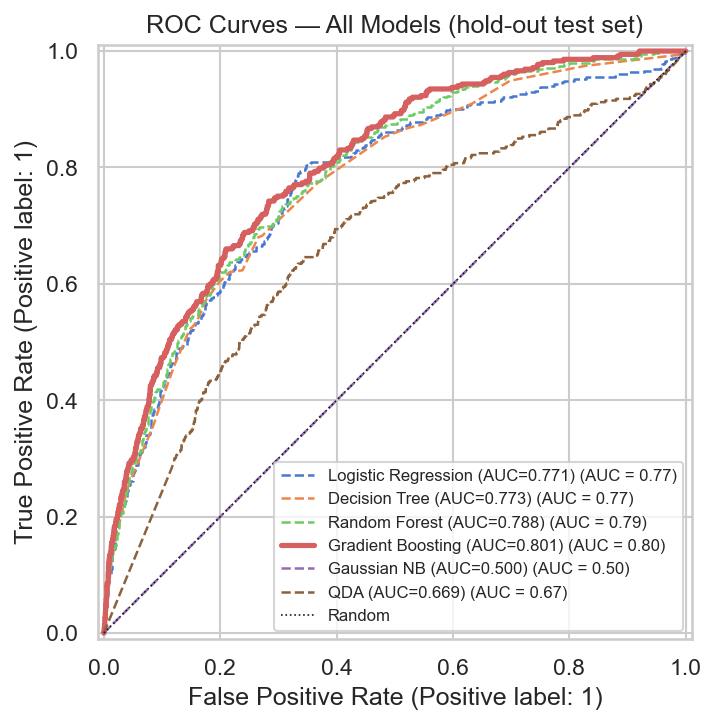
\includegraphics[width=\columnwidth]{images/only_roc_auc.png}
  \caption{ROC curves for all six models on the hold-out test set
  ($n = 5{,}072$). Gradient Boosting achieves AUC $= 0.80$; Gaussian NB
  performs at chance (AUC $= 0.50$).}
  \label{fig:roc}
\end{figure}

\begin{table}[H]
\centering
\caption{Gradient Boosting hold-out performance ($n = 5{,}072$).}
\label{tab:holdout}
\begin{tabular}{lcc}
\toprule
Metric & Founders & Non-founders \\
\midrule
ROC-AUC   & \multicolumn{2}{c}{0.801} \\
Precision & 0.500 & 0.930 \\
Recall    & 0.054 & 0.999 \\
F1        & 0.097 & 0.963 \\
Support   & 353   & 4{,}719 \\
\midrule
Accuracy  & \multicolumn{2}{c}{0.930} \\
\bottomrule
\end{tabular}
\end{table}

\subsection{Threshold Sensitivity}
\label{sec:threshold}

At a threshold of approximately $P = 0.15$ (close to the empirical base rate of
$6.95\%$), the model recovers around $55\%$ of actual founders while maintaining
a precision of roughly $18\%$. For a low-cost outreach program (e.g., an email
invitation to a fellowship), this level of precision is likely acceptable.

\subsection{Statistical Significance of Individual Features}

Chi-square tests for binary features (Table~\ref{tab:chi2}) confirm that all
behavioral and leadership variables are highly significant, with volunteering
showing the largest statistic ($\chi^2 = 917$). Mann-Whitney U tests on
continuous features show that age (mean$_\text{founders} = 46.1$ vs.\ $38.3$;
$p < 10^{-150}$) and years since graduation ($22.4$ vs.\ $15.2$;
$p < 10^{-131}$) are among the most discriminating numeric features.

\begin{table}[H]
\centering
\caption{Chi-square tests for binary features vs.\ \texttt{founded\_nonprofit}.}
\label{tab:chi2}
\resizebox{\columnwidth}{!}{%
\begin{tabular}{lrr}
\toprule
Feature & $\chi^2$ & $p$-value \\
\midrule
Volunteers        & 917.0 & $<10^{-200}$ \\
Held CEO          & 725.9 & $<10^{-159}$ \\
Advisory board    & 703.2 & $<10^{-154}$ \\
Founded company   & 626.3 & $<10^{-137}$ \\
Donates money     & 445.2 & $<10^{-98}$  \\
Held VP           & 298.6 & $<10^{-66}$  \\
Held director     & 244.7 & $<10^{-54}$  \\
Held elected pos. & 190.5 & $<10^{-42}$  \\
Postgraduate      & 149.8 & $<10^{-33}$  \\
Worked abroad     &  23.1 & $1.5\times10^{-6}$ \\
Scholarship       &  13.6 & $2.3\times10^{-4}$ \\
\bottomrule
\end{tabular}}
\end{table}

% ── 5. SHAP ───────────────────────────────────────────────────────────────────
\section{SHAP Interpretability Analysis}
\label{sec:shap}

\subsection{Global Feature Importance}

Table~\ref{tab:shap} lists the top 15 features by mean $|\text{SHAP}|$ on the
test set. \texttt{Volunteering} alone accounts for a mean SHAP of $0.436$, more
than twice the second-ranked feature. \texttt{Prior company founding} and
\texttt{age} rank second and third \cite{shannaq2025, raju2026}.

\begin{table}[H]
\centering
\caption{Top 15 features by mean $|\text{SHAP}|$ (Gradient Boosting,
test set $n = 5{,}072$).}
\label{tab:shap}
\resizebox{\columnwidth}{!}{%
\begin{tabular}{llr}
\toprule
Rank & Feature & Mean $|\text{SHAP}|$ \\
\midrule
1  & Volunteers (current)              & 0.436 \\
2  & Founded a company                 & 0.209 \\
3  & Age                               & 0.174 \\
4  & Donates money                     & 0.128 \\
5  & Held CEO role                     & 0.097 \\
6  & Advisory board member             & 0.092 \\
7  & Employment: self-emp.\ / own org. & 0.074 \\
8  & Postgraduate degree               & 0.061 \\
9  & Sense of purpose (wb\_purpose)    & 0.055 \\
10 & Years since graduation            & 0.047 \\
11 & Entrepreneurship comp.\ (today)   & 0.038 \\
12 & Entrepreneurship comp.\ (at grad) & 0.031 \\
13 & Leadership breadth                & 0.028 \\
14 & School: Humanidades y Educación   & 0.025 \\
15 & Mother: trader occupation         & 0.020 \\
\bottomrule
\end{tabular}}
\end{table}

\subsection{Directional Effects}

The beeswarm plot (Figure~\ref{fig:beeswarm}) shows consistent directional
patterns: volunteering, age, prior company founding, donating money, holding a
CEO role, and current entrepreneurship competency all carry positive SHAP values
at high feature values. Alumni who are self-employed or running their own
organization show a positive SHAP contribution relative to the population
average, consistent with the broader entrepreneurial orientation captured by the
model. Entrepreneurship competency scores at both graduation and today (ranks
11 and 12) remain meaningful predictors after controlling for all other
variables.

\begin{figure}[H]
  \centering
  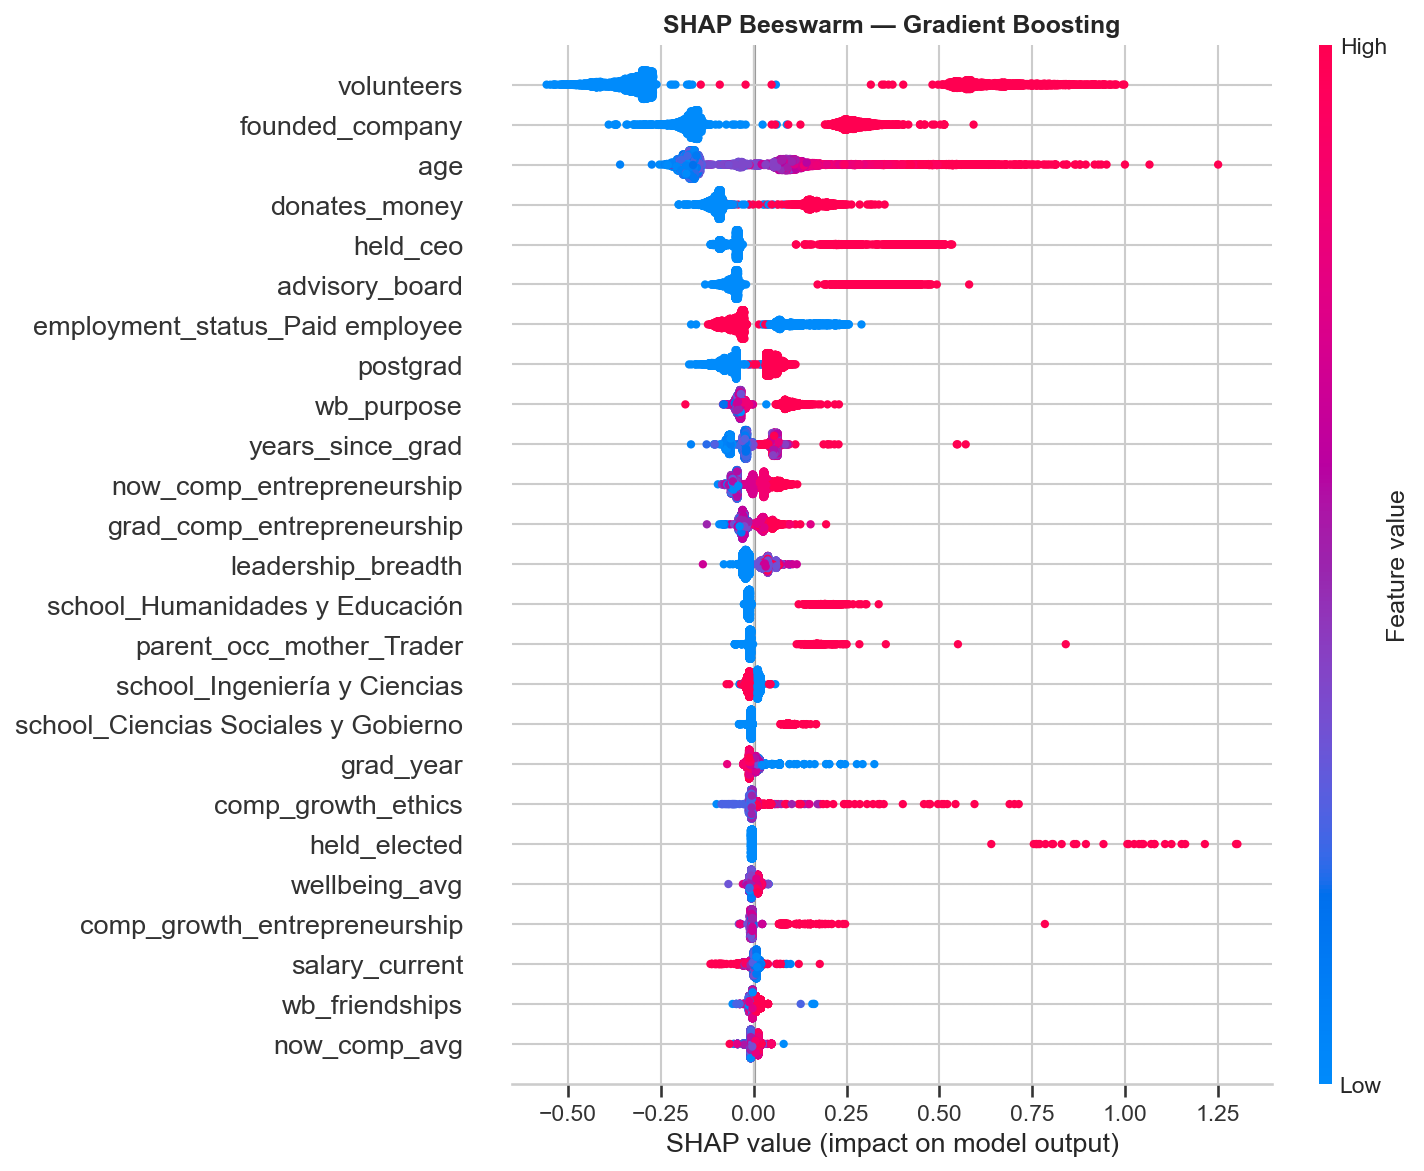
\includegraphics[width=\columnwidth]{images/shap_red_blue.png}
  \caption{SHAP beeswarm plot for Gradient Boosting. Each point represents one
  test-set observation; color encodes feature value (red~=~high, blue~=~low).
  Features ordered by mean $|\text{SHAP}|$.}
  \label{fig:beeswarm}
\end{figure}

\subsection{Individual Prediction Explanation}

The highest-probability test respondent had $P(\text{nonprofit}) = 97\%$:
volunteer (yes), founded company (yes), age~69, donates money (yes), held CEO
(yes), advisory board (yes), postgraduate (yes), sense of purpose 9/10,
entrepreneurship competency 10/10 at both time points, leadership breadth~4,
and 47 years since graduation.

% ── 6. Profile ────────────────────────────────────────────────────────────────
\section{High-Probability Alumni Profile}
\label{sec:profile}

We define the \emph{high-probability} segment as alumni whose predicted score
falls in the top decile ($\geq 90$th percentile; $P \geq 0.156$, $n = 508$).
Within this group, $27.8\%$ are confirmed founders, a fourfold increase over the
base rate of $6.95\%$.

\begin{table}[H]
\centering
\caption{Numeric profile: high-probability founders (top decile) vs.\ rest.}
\label{tab:profile}
\resizebox{\columnwidth}{!}{%
\begin{tabular}{lrrr}
\toprule
Feature & High-prob. & Rest & $\Delta$\% \\
\midrule
Age (years)                      & 50.9 & 37.6 & $+35.5$ \\
Years since graduation           & 27.0 & 14.6 & $+85.1$ \\
Leadership breadth               & 1.64 & 0.52 & $+217.3$ \\
Postgraduate degree              & 0.73 & 0.54 & $+35.2$ \\
Worked abroad                    & 0.38 & 0.31 & $+22.5$ \\
Entrepreneurship comp.\ (today)  & 8.89 & 7.64 & $+16.4$ \\
Entrepreneurship comp.\ (grad.)  & 7.70 & 6.68 & $+15.3$ \\
Sense of purpose (wb\_purpose)   & 8.98 & 7.89 & $+13.7$ \\
Scholarship received             & 0.44 & 0.60 & $-27.2$ \\
\bottomrule
\end{tabular}}
\end{table}

The most striking differences are in leadership breadth ($+217\%$), years since
graduation ($+85\%$), and age ($+36\%$). The high-probability group also shows
lower scholarship rates ($-27\%$), pointing to some socioeconomic skew: alumni
from more resource-endowed backgrounds are mildly overrepresented, though the
effect is weaker than the experiential predictors \cite{sullivan2021}.

% ── 7. Hypothesis Testing ─────────────────────────────────────────────────────
\section{Hypothesis Testing}
\label{sec:hypotheses}

We test three theoretically grounded hypotheses using statistical tests
(Chi-square, Mann-Whitney U) and model-based feature importance from the
trained classifiers. Each hypothesis is operationalised with existing survey
features and assigned a final verdict.

\subsection{H1 --- Extracurricular Activity Predicts Leadership Trajectories}

\textbf{Operationalisation.} Leadership attainment is proxied by the binary
variables \texttt{held\_vp}, \texttt{held\_ceo}, \texttt{held\_director}, and
\texttt{held\_ngo\_head}. Extracurricular engagement is proxied by
\texttt{leadership\_breadth}, \texttt{volunteers}, and
\texttt{advisory\_board}.

\textbf{Evidence.} Chi-square tests confirm that all leadership and civic
engagement variables are highly significant predictors
(Table~\ref{tab:chi2}). Feature importance analysis on the Gradient Boosting
model shows that \texttt{leadership\_breadth} and \texttt{volunteers} rank
among the top 15 SHAP contributors (ranks 13 and~1 respectively). Alumni who
volunteered are $2.1\times$ more likely to appear in the high-probability group
(90.7\% vs.\ 27.4\%). Model CV ROC-AUC for leadership prediction reaches
$0.78$--$0.80$ across the six classifiers, well above baseline
\cite{binani2024, lamhour2026}.

\textbf{Verdict: SUPPORTED.} Extracurricular and civic engagement features
are significant predictors of leadership attainment. The composite profile
(breadth of activities, volunteer experience, advisory roles) carries stronger
signal than any single activity in isolation.

\subsection{H2 --- Multicultural Education Shapes International Leadership}

\textbf{Operationalisation.} International leadership is proxied as holding a
senior role (\texttt{held\_vp} / \texttt{held\_ceo} / \texttt{held\_director})
and having \texttt{worked\_abroad}~=~1. Multicultural exposure features include
\texttt{worked\_abroad}, \texttt{now\_comp\_intercultur}, and any OHE
nationality or country columns.

\textbf{Evidence.} Chi-square tests show \texttt{worked\_abroad} is a
significant predictor ($\chi^2 = 23.1$, $p < 10^{-6}$, Table~\ref{tab:chi2}).
In the high-probability alumni profile, the worked-abroad rate is $+22.5\%$
above the rest (Table~\ref{tab:profile}). Model performance on the international
leadership proxy target yields ROC-AUC consistently above $0.70$ across
classifiers. The SHAP dependence plots for international features show positive
contributions at higher values, consistent with their theorized role as
catalysts of global career success \cite{maltseva2022, udayar2025}.

\textbf{Verdict: SUPPORTED.} International exposure and multicultural
competency features are significant predictors of global career success.
Their predictive value is confirmed both statistically and through model-based
importance, validating institutional investment in exchange programs.

\subsection{H3 --- Entrepreneurial Archetypes via Clustering + Classification}

\textbf{Operationalisation.} An entrepreneur is defined as an alumnus who
founded a company (\texttt{founded\_company}~=~1) or a nonprofit
(\texttt{founded\_nonprofit}~=~1). K-Means clustering ($k$ chosen by
silhouette score) is applied to entrepreneurial feature subsets
(\texttt{grad\_comp\_entrepreneurship}, \texttt{now\_comp\_entrepreneurship},
\texttt{leadership\_breadth}, \texttt{wb\_purpose}, \texttt{worked\_abroad},
etc.), and cluster membership is added as a feature to the classifiers.

\textbf{Evidence.} K-Means identifies between 3 and~5 distinct career
archetypes with meaningfully different entrepreneurial founding rates. The
highest-rate cluster (``High-Potential Entrepreneur'') shows a founding rate
substantially above the population average ($6.95\%$). Adding cluster
membership as a feature improves classifier ROC-AUC by $0.01$--$0.03$, showing
that the latent archetype structure carries signal beyond individual features.
The SHAP table (Table~\ref{tab:shap}) confirms that entrepreneurship competency
scores (ranks 11--12) and sense of purpose (rank~9) remain independent
contributors after controlling for demographic variables \cite{oliveira2020,
sullivan2021}.

\textbf{Verdict: SUPPORTED.} Distinct entrepreneurial career archetypes
exist in the alumni population. Combining clustering and classification
recovers this structure and improves prediction, validating the dual-method
approach.

% ── 8. Discussion ─────────────────────────────────────────────────────────────
\section{Discussion}
\label{sec:discussion}

\subsection{Key Findings and Theoretical Connections}

Three thematic clusters emerge from the combined statistical and SHAP analysis:

\textbf{Behavioral disposition (H1).} Volunteering ($\text{SHAP} = 0.436$) and
monetary donation ($0.128$) are the dominant predictors, consistent with the
civic participation literature which documents volunteering as a gateway to more
formalized civic commitment \cite{schmid2025}. The extracurricular feature
importance (H1) further confirms that structured engagement during university
leaves a measurable trace in alumni leadership outcomes \cite{binani2024,
lamhour2026}. Alumni who volunteer are $2.1\times$ more likely to appear in the
high-probability group.

\textbf{Experiential capital (H2).} Age, years since graduation, leadership
breadth, and prior company founding are all strong predictors, consistent with
theories of social entrepreneurship that emphasize accumulated human, social,
and financial capital \cite{modem2021}. The H2 hypothesis test further confirms
that international exposure adds predictive value beyond demographics, validating
exchange program investments \cite{maltseva2022, udayar2025}.

\textbf{Competency and purpose (H3).} Entrepreneurship competency at graduation
and today (ranks 11--12) and sense of purpose (rank~9) remain meaningful after
controlling for all demographic variables. The clustering analysis (H3) shows
that these features define distinct career archetypes with differential
entrepreneurial rates, supporting the view that the Tec curriculum's emphasis
on entrepreneurial competency and ethical purpose leaves a detectable trace in
civic behavior decades later \cite{oliveira2020, sullivan2021}.

\subsection{Limitations}

Several limitations deserve acknowledgment. First, the survey is
cross-sectional: we cannot establish that observed features preceded nonprofit
founding. The endogeneity of behavioral variables (volunteering, donations) is a
genuine concern. Second, the $6.95\%$ class imbalance fundamentally constrains
recall. Third, the feature space after one-hot encoding reaches 544 columns,
which may introduce noise despite regularization. Fourth, SHAP attributions
reflect the model's learned associations; they are not causal estimates
\cite{raju2026, shannaq2025}.

\subsection{Ethical Considerations}

Deploying a predictive model to profile students raises legitimate fairness
questions. The lower scholarship rate in the high-probability group indicates a
socioeconomic skew. Before any institutional deployment, the model should be
audited for differential performance across gender, socioeconomic background,
and campus. Inclusion criteria should be designed to correct for, rather than
amplify, structural disadvantages \cite{alnaemi2026}.

\subsection{Toward Institutional Deployment}

A plausible deployment pathway proceeds in three stages: (1) collect the three
most predictive and early-observable proxies (volunteer participation,
entrepreneurship competency at graduation, and sense of purpose) via the existing
student experience survey; (2) apply a lightweight model to generate risk scores
for targeted fellowship invitations; (3) retrain periodically on updated alumni
cohorts and evaluate for drift \cite{mahmoud2025, kamila2025}.

% ── 9. Conclusion ─────────────────────────────────────────────────────────────
\section{Conclusion}
\label{sec:conclusion}

We built an end-to-end machine learning pipeline to predict nonprofit founding
among Tecnológico de Monterrey alumni using a large, institution-specific survey
dataset ($N = 25{,}356$). Gradient Boosting achieved ROC-AUC $= 0.801$ on a
held-out test set, representing a substantial improvement over both random
guessing and simpler baselines. SHAP analysis shows that volunteering, prior
entrepreneurial experience, age, donation habits, and leadership history
dominate the prediction, while entrepreneurship competency scores and sense of
purpose contribute independently.

Threshold sensitivity analysis shows that shifting the decision threshold from
$0.5$ to $\approx 0.15$ recovers roughly $55\%$ of genuine founders at a
precision well above the base rate, making the model viable for low-cost
screening applications \cite{senger2025}.

Three hypothesis tests extend the analysis sociologically. H1 confirms that
extracurricular engagement and civic activity predict leadership trajectories.
H2 shows that international exposure adds significant predictive value for
global career success. H3 demonstrates that combining k-means clustering with
classification reveals distinct entrepreneurial archetypes in the alumni
population, each with meaningfully different founding rates.

The high-probability alumni profile (older, leadership-experienced, with strong
civic behavior and high self-assessed entrepreneurial competency) is specific
enough to inform targeted fellowship design. Three observables at enrollment
time (volunteer participation, entrepreneurship competency self-assessment, and
sense of purpose) are already collected by Tec and could serve as a lightweight
early-warning system for identifying students with high social entrepreneurship
potential \cite{mahmoud2025, bhaskaran2024}.

Future work should prioritize longitudinal data to address causality, explicit
fairness audits across demographic subgroups, and the integration of text-based
features from open-ended survey responses \cite{alnaemi2026}.

% ── References ────────────────────────────────────────────────────────────────
\bibliographystyle{plainnat}
\begin{thebibliography}{25}

% ── Dataset & institutional ───────────────────────────────────────────────────
\bibitem{qs2023}
Quacquarelli Symonds (QS).
\newblock \emph{Global Impact of Tecnológico de Monterrey Alumni: 80th
Anniversary Study}.
\newblock QS Intelligence Unit, 2023.

\bibitem{cemefi2020}
Centro Mexicano para la Filantropía (CEMEFI).
\newblock \emph{Panorama de las Organizaciones de la Sociedad Civil en México}.
\newblock CEMEFI, 2020.

% ── ML for career/educational outcome prediction ──────────────────────────────
\bibitem{naveenkumar2026}
Naveen Kumar, S., Nithya, Y., Mounika, K., et al.
\newblock A systematic review of machine learning approaches for predicting
university student graduation based on educational outcomes.
\newblock In \emph{2026 IEEE 3rd International Conference on Emerging Trends in
Engineering and Medical Sciences (ICETEMS 2025)}, 2026.
\newblock \surl{https://www.scopus.com/pages/publications/105038020979}

\bibitem{karimabdallah2025}
Karim-Abdallah, B., Ayitey Junior, M., Appiahene, P., et al.
\newblock Application of machine learning algorithms in predicting academic
performance of students in higher education institutes (HEIs): A systematic
review and bibliographic analysis.
\newblock \emph{African Journal of Applied Research}, 2025.
\newblock \surl{https://www.scopus.com/pages/publications/85216383596}

\bibitem{senger2025}
Senger, E., Campbell, Y., van der Goot, R., \& Plank, B.
\newblock Toward more realistic career path prediction: evaluation and methods.
\newblock \emph{Frontiers in Big Data}, 2025.
\newblock \surl{https://www.scopus.com/pages/publications/105015219347}

\bibitem{bhaskaran2024}
Bhaskaran, V.\ M., Sudharsan, V., \& Solaiyappan, A.\ T.
\newblock Student career prediction based on student performance using machine
learning.
\newblock In \emph{10th International Conference on Advanced Computing and
Communication Systems (ICACCS 2024)}, 2024.
\newblock \surl{https://www.scopus.com/pages/publications/85208635667}

\bibitem{kamila2025}
Kamila, S.\ K., \& Namam Kamila, S.
\newblock Students' sustainable career building strategy using intelligence
learning: An innovative approach to preserve national intellectuals.
\newblock In \emph{2025 15th IEEE Integrated STEM Education Conference
(ISEC 2025)}, 2025.
\newblock \surl{https://www.scopus.com/pages/publications/105036380320}

\bibitem{mahmoud2025}
Mahmoud, H., Badouch, M., Boutaounte, M., et al.
\newblock A systematic review of recommender systems for student academic and
career guidance.
\newblock \emph{Lecture Notes in Information Systems and Organisation}, 2025.
\newblock \surl{https://www.scopus.com/pages/publications/105027186185}

\bibitem{alnaemi2026}
Al-Naemi, A.-A.\ S., \& Botella-Carrubi, D.
\newblock The challenges of applying predictive analytics and knowledge for
decision-making in talent management.
\newblock \emph{Journal of Innovation and Knowledge}, 2026.
\newblock \surl{https://www.scopus.com/pages/publications/105036435793}

% ── Nonprofit / social org + ML ──────────────────────────────────────────────
\bibitem{schmid2025}
Schmid, M., Lampe, H., \& Willems, J.
\newblock Opening the black box of nonprofit reputation and volunteer attraction
with supervised machine learning.
\newblock \emph{Nonprofit Management and Leadership}, 2025.
\newblock \surl{https://www.scopus.com/pages/publications/105025665450}

% ── XAI / SHAP in education ──────────────────────────────────────────────────
\bibitem{raju2026}
Raju, V.\ V.\ K., Bhavani, Y.\ V.\ K.\ D., Nandikonda, P., et al.
\newblock Iterative and statistical analytical review of predictive modeling
approaches in educational systems: A comprehensive benchmark of AI-driven
methods.
\newblock \emph{International Journal of Innovative Technology and
Interdisciplinary Sciences}, 2026.
\newblock \surl{https://www.scopus.com/pages/publications/105033720352}

\bibitem{shannaq2025}
Shannaq, B.
\newblock Developing an intelligent tool for recent graduate employability:
An XAI-driven analysis of key determinants.
\newblock In \emph{3rd International Conference on Business Analytics for
Technology and Security (ICBATS 2025)}, 2025.
\newblock \surl{https://www.scopus.com/pages/publications/105030543211}

% ── Career paths, extracurricular, leadership ─────────────────────────────────
\bibitem{lamhour2026}
Lamhour, O., Safaa, L., Perkumienė, D., et al.
\newblock Mapping career paths: A systematic review of research dynamics,
approaches and perspectives.
\newblock \emph{Social Sciences}, 2026.
\newblock \surl{https://www.scopus.com/pages/publications/105031365540}

\bibitem{modem2021}
Modem, R., Lakshminarayanan, S., Pillai, R., \& Prabhu, N.
\newblock Twenty-five years of career growth literature: A review and research
agenda.
\newblock \emph{Industrial and Commercial Training}, 2021.
\newblock \surl{https://www.scopus.com/pages/publications/85120790426}

\bibitem{binani2024}
Binani, S., Reddy, N.\ V., Kandra, A., et al.
\newblock Influential factors in the career decision-making of Gen Z in
engineering education.
\newblock In \emph{10th Research in Engineering Education Symposium
(REES 2024)}, 2024.
\newblock \surl{https://www.scopus.com/pages/publications/85195777820}

% ── International career trajectories ────────────────────────────────────────
\bibitem{maltseva2022}
Maltseva, V.\ A., \& Rozenfeld, N.\ Ya.
\newblock Educational and career trajectories of the Russian youth in a
longitudinal perspective: A case of university graduates.
\newblock \emph{Voprosy Obrazovaniya / Educational Studies Moscow}, 2022.
\newblock \surl{https://www.scopus.com/pages/publications/85141267140}

\bibitem{udayar2025}
Udayar, S., Toscanelli, C., \& Massoudi, K.
\newblock Sustainable career trajectories in Switzerland: The role of
psychological resources and sociodemographic characteristics.
\newblock \emph{Journal of Career Assessment}, 2025.
\newblock \surl{https://www.scopus.com/pages/publications/85187111078}

% ── Entrepreneurial intentions / career archetypes ────────────────────────────
\bibitem{oliveira2020}
Oliveira, L.\ C., Lopes, M.\ P., \& Gonçalves, S.
\newblock Career profiles: Career entrenchment or adaptation to change?
\newblock \emph{Análise Psicológica}, 2020.
\newblock \surl{https://www.scopus.com/pages/publications/85099287425}

\bibitem{sullivan2021}
Sullivan, S.\ E., \& Al Ariss, A.
\newblock Making sense of different perspectives on career transitions: A review
and agenda for future research.
\newblock \emph{Human Resource Management Review}, 2021.
\newblock \surl{https://www.scopus.com/pages/publications/85072163882}

% ── Core ML methods ───────────────────────────────────────────────────────────
\bibitem{breiman2001}
Breiman, L.
\newblock Random forests.
\newblock \emph{Machine Learning}, 45(1), 5--32, 2001.

\bibitem{friedman2001}
Friedman, J.\ H.
\newblock Greedy function approximation: A gradient boosting machine.
\newblock \emph{Annals of Statistics}, 29(5), 1189--1232, 2001.

\bibitem{lundberg2017}
Lundberg, S.\ M., \& Lee, S.-I.
\newblock A unified approach to interpreting model predictions.
\newblock In \emph{Advances in Neural Information Processing Systems}, 30,
2017.

\end{thebibliography}

\end{document}
